%==============================================================================================================================================
%==============================================================================================================================================

\subsection{A B-spline representation for pp functions}

\subfile{chapter-3-subfiles/chapter-3-bspline-representation}


%==============================================================================================================================================

\subsection{Single-regressor varying coefficient models via B-spline basis expansions}

\subfile{chapter-3-subfiles/chapter-3-bspline-single-index-vc-models}

%==============================================================================================================================================

%%==============================================================================================================================================
%%==============================================================================================================================================
%%==============================================================================================================================================


\subsection{P-spline estimators for regularized estimation of fitted curves}

\subfile{chapter-3-subfiles/chapter-3-pspline-models-intro}

 %%==============================================================================================================================================
 
 \subsubsection{Difference penalties}
 \subfile{chapter-3-subfiles/chapter-3-pspline-difference-penalties}

%==============================================================================================================================================


\subsubsection{P-splines for single-index VC models}
 \subfile{chapter-3-subfiles/chapter-3-single-index-pspline-vc-models}

%%====================================================================================

\subsection{Properties of P-splines}
 \subfile{chapter-3-subfiles/chapter-3-properties-of-psplines}


%%====================================================================================
\subsection{The reguarlized MLE for $\phi$ via tensor product P-splines}
 \subfile{chapter-3-subfiles/chapter-3-tensor-product-pspline-MLE}


%We employ maximum likelihood  for the estimation of  the varying coefficient function $\phi\left(t,s\right)$ and the innovation variance function $\sigma\left(t\right)$, though neither the derivation the form of model~\ref{eq:ARmodel} nor model~\ref{eq:MyModel} via the Cholesky decomposition rely on any assumptions about the distribution of $Y$. 
%
%For fixed $\left\{ \sigma_j^2 \right\}$, as a function of $\phi_{jk}$ the negative log-likelihood for a sample of $N$  i.i.d. observations $Y_1,Y_2,\dots,Y_N$ from a multivariate Gaussian distribution is proportional to the usual error sums of squares:
%
%\begin{equation}
%-2 L\left(y_1,\dots,y_N ,\phi \vert \vsigmasq \right) \propto \sum_{i=1}^N \sum_{j=2}^{m_i} \sigma\left({t_j}\right)^{-2} \left(y_{ij} - \sum_{k=1}^{j-1}\phi\left({t_{ij},t_{ik}}\right)y_{ik} \right)^2 \label{loglikelihood}
%\end{equation}
%\noindent
%where 
%\[
%y_i = \left( y_{i1}, y_{i2}, \dots, y_{i,m_i}\right), \quad i=1,\dots,N 
%\] 
%
%%% explain here that we omit y_{i1} from the likelihood here because in the first stage of estimation (for $\phi$), the first observation in each vector doesn't contribute to the likelihood
%\noindent
%denotes the vector of observations for subject $i$ with corresponding measurement times 
%\[
%t_{i1} < t_{i2} < \dots < t_{i,m_i}.
%\]
%The form of the likelihood of $y_1,\dots,y_N$ indicates that we allow both the number of measurements as well as the observation times to varying across subjects. The $\left\{t_{ij} \right\}$ need not be evenly-spaced within or across individuals. Denote the innovation variance function evaluated at the vector of observed time points by $\vsigmasq$, and similarly let $\vphistar$ denote the resulting vector when evaluating $\phi$ at the observed grid of time points, transformed to the $l$-$m$ axis. Estimation of the varying coefficient function and the innovation variance function may be accomplished in an iterative fashion:
%
%\fbox{\parbox{\textwidth}{\begin{enumerate}
%\item Fix $\vsigmasq = \vsigmasq_0$;
%\item find $\widehat{\vphistar} = \underset{\vphistar}{\arg\max} -2 L\left(y_1,\dots,y_N ,\vphistar \vert \vsigmasq_0 \right)$.
%\item Fix $\vphistar= \widehat{\vphistar}$;
%\item find $\widehat{\vsigmasq} = \underset{\vsigmasq}{\arg\max} -2 L\left(y_1,\dots,y_N , \vsigmasq \vert \widehat{\vphistar} \right)$.
%\item Iterate until convergence.
%\end{enumerate}}}
%
%\vspace{0.5cm}


% 
%\section{\emph{Penalized maximum likelihood estimation}}
%
%\begin{enumerate}
%\item Fix $\sigma_{ij}^2 = \sigma_{ij0}^2$, $i=1,\dots,N$ ,$j=1,\dots,M$.
%\item Find $\phi_0 = \underset{\phi}{arg \; min} -2L_\phi\left(\phi, y_1,\dots, y_N \right) + \lambda J\left( \phi \right)$
%\item Fix $\phi = \phi_{0}$.
%\item Find  $\sigma_{0}^2 = \underset{\sigma^2}{arg\; min} -2L_\sigma^2\left(\sigma^2, y_1,\dots, y_N \right) + \lambda J\left( \sigma^2 \right)$
%\end{enumerate}
%
%\begin{adjustwidth}{-2cm}{-2cm}
%\begin{equation}
%-2 L_\phi\left(\phi, y_1, \dots,y_N \right) = \sum_{i=1}^N \sum_{j=2}^{m_i} \sigma_{ij0}^{-2} \left(y_{ij} - \sum_{k=1}^{j-1}\phi\left({t_{ij},t_{ik}}\right)y_{ik} \right)^2 \label{loglikelihood}
%\end{equation}
%\end{adjustwidth}
% 





% 
%\section{\emph{Smooth ANOVA models}}
%Decompose
%\begin{equation} \label{eq:SANOVA-model}
%\carrotorangemath{
%\phi\left(l,m\right) = \mu + \phi_1\left(l\right) + \phi_2\left(m\right) + \phi_{12}\left(l,m\right)},
%\end{equation} 
%so Model~\ref{eq:MyModel} becomes
%
%\begin{align*}  
%\begin{split}% \label{eq:expanded-ps-anova-vc-model}
% y\left(t_j \right)  = \sum_{k=1}^{j-1} \bigg[\mu + \phi_1\left(l_{jk}\right) +  &\phi_2\left(m_{jk}\right) \bigg.\\[-2ex]
%\bigg. &+ \phi_{12}\left(l_{jk},m_{jk}\right) \bigg]y\left(t_k\right)+ \sigma\left(t_j\right)e\left({t_j}\right)
%\end{split}
%\end{align*}
% 

% \begin{columns}
%\begin{column}{0.5\textwidth}
%Equip $l$ and $m$ with
%\begin{align*}
%B_{1}\left(l\right),\dots, B_{K}\left(l\right),\\
%B_{1}\left(m\right),\dots, B_{L}\left(m\right)
%\end{align*}
%to build
%\begin{equation*}
%T_{jk}\left(l,m\right) = B_j\left(l\right){B}_k\left(m\right)
%\end{equation*}
%  \end{column}
%\begin{column}{0.5\textwidth}  %%<--- here
%    \begin{center}
%    \begin{figure}
%    \graphicspath{{img/}}
% 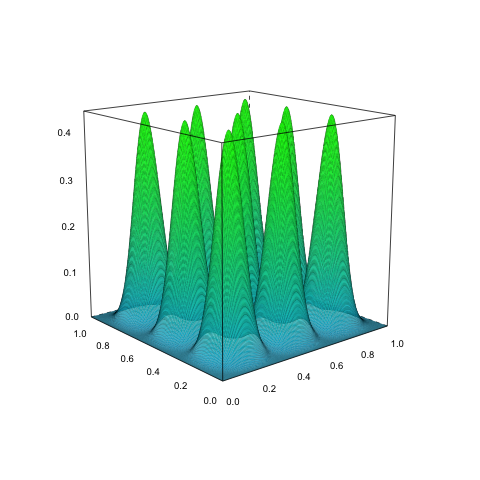
\includegraphics[width=4cm]{sparse_bicubic_basis}
% \caption{A ``thinned'' tensor product basis}
% \end{figure}
%     \end{center}
%\end{column}
%\end{columns}
%\vspace{0.3cm}
%\begin{equation*}
%\phi\left(l,m\right) = \sum_{i=1}^K \sum_{j=1}^L \theta_{ij} B_{i}\left(l\right) B_{j}\left(m\right)
%\end{equation*}
%
 
%The parameters of the functional autoregressive model given by \ref{eq:MyModel} define the elements of the precision matrix $\Omega$, rather than the elements of $\Sigma$ itself. It is well known that if we let $Y = \left(Y_1, \dots, Y_m\right)^\prime$ denote the random vector having joint distribution with mean zero and covariance matrix $\Sigma$, then the elements of $\Sigma^{-1}=\Omega$, $\left\{ \omega_{ij} \right\}$ may be interpreted as partial covariances between the elements of $Y$. This suggests shrinking $\phi$ to zero for large values of $l$. One can show that if $T$ has $k$ non-zero diagonals, then the middle $k$ diagonals of $\Sigma^{-1}$ are non-zero.  

%For ease of exposition, we first focus our attention on the estimation of $\phi$ assume that $\sigma^2\left(t\right)$ is fixed and known. Estimation of the innovation variance function is presented in Section~\ref{section:variance-estimation}. In the case that subjects share a common set of observation times $t_1 < \dots < t_m$,  it is well known that the MLE for $\Sigma$, $S = \sum_{i=1}^N y_i y_i^\prime$ is highly unstable in high dimensions, a condition that is potentially worsened when one or more subjects has at least one observation time that is unique from the set of observation times common across subjects. To mitigate instability due to high dimensionality and simultaneously permit the estimation of $\phi\left(\cdot,\cdot\right)$ as a smooth bivariate function, we obtain a covariance estimator by applying bivariate smoothing of the elements of the Cholesky factor. 
%
%Estimating the varying coefficient function $\phi$, however, is quite different from the usual problem of estimating an arbitrary bivariate function. In the case of the latter, we most typically treat both arguments equally in terms of regularization, but in the case of covariance estimation and the generalized coefficient function equal treatment of $l$ and $m$ in terms of penalization perhaps is not the most appropriate approach. The lag component, $l$, has particularly significant meaning in terms of the covariance function and thus also in terms of $\phi$ and is of considerable more interest than the orthogonal component, $m$. We parameterize $\phi$ in terms of the transformed domain:
%
%\begin{align*}
%l = t-s, \qquad m = \frac{1}{2}\left(s+t\right),
%\end{align*}
%\noindent
%so that the following relationship holds:
%\begin{align*}
%\phi\left(s,t\right) = \phi\left(s-t, \frac{1}{2}\left(s+t\right)\right) =\phi\left(l,m\right)
%\end{align*}
%with 
%\begin{equation} \label{eq:phi-star-domain}
%\frac{l}{2} < m < 1 - \frac{l}{2}, \quad 0 < l < 1.
%\end{equation}
%
%\noindent
%The likelihood can be written in terms of the reparameterized varying coefficient function:
%
%\begin{align} 
%\begin{split} \label{loglikelihood}
%-2L\left(y_1,\dots,y_N ,\phi \vert \vsigmasq \right) &= \sum_{i=1}^n \sum_{j=2}^{m_i} \sigma_{ij}^{-2} \left(y_{ij} - \sum_{k=1}^{j-1}\phi\left({t_{ij},t_{ik}}\right)y_{ik} \right)^2 \\
%&= \sum_{i=1}^n \sum_{j=2}^{m_i} \sigma_{ij}^{-2} \left(y_{ij} - \sum_{k=1}^{j-1}\phi\left({l_{ijk},m_{ijk}}\right)y_{ik} \right)^2 
%\end{split} 
%\end{align}

%%====================================================================================

\subsection{Model selection and tuning parameter estimation}

\subfile{chapter-3-subfiles/chapter-3-tensor-product-pspline-model-selection}

